\documentclass[11]{article}
\usepackage[margin=1in]{geometry}
\usepackage{amsmath,amssymb,amsthm,enumitem}
\usepackage{fullpage}
\usepackage{tikz}
\usepackage[latin1]{inputenc}
\usetikzlibrary{arrows,shapes.gates.logic.US,shapes.gates.logic.IEC,calc,trees}
\usepackage{xcolor}
\usepackage{listings}

\definecolor{comment}{rgb}{0.0, 0.5, 0.0}

\lstdefinestyle{CStyle}{
    backgroundcolor=\color{lightgray},   
    commentstyle=\color{comment},
    keywordstyle=\color{blue},
    numberstyle=\tiny\color{black},
    stringstyle=\color{violet},
    basicstyle=\footnotesize,
    breakatwhitespace=false,         
    breaklines=true,                 
    captionpos=b,                    
    keepspaces=true,                 
    numbers=left,                    
    numbersep=5pt,                  
    showspaces=false,                
    showstringspaces=false,
    showtabs=false,                  
    tabsize=2,
    language=C
}

\begin{document}

\tikzstyle{branch}=[fill,shape=circle,minimum size=3pt,inner sep=0pt]

\begin{titlepage}
\begin{center}
\vspace*{2cm}
\Large{\textbf{EECE 5643: Simulation and Performance Evaluation}}\\
\Large{\textbf{Professor Ningfang Mi}}\\
\vfill
\line(1,0){400}\\[1mm]
\huge{\textbf{Homework 3}}\\[3mm]
\Large{\textbf{- Assignment Due: 02/16/2023 -}}\\[1mm]
\line(1,0){400,0}\\
\vfill
Harrison Sun\\
Monday, Thursday 11:45 am - 1:25 pm \\
Completed: \today\
\end{center}
\end{titlepage}

\section{\textbf{Ex. 3.1.1}}
\textbf{(a) Modify program ssq2 to use $Exponential(1.5)$ service times.}\\
\textbf{(b) Process a relatively large number of jobs, say 100000, and report what changes this produces relative to the statistics in Example 3.1.3.}\\
\textbf{(c) Explain (or conjecture) why some statistics change and others do not.}\\

\begin{table}[h]
\centering
\begin{tabular}{l|lllll}
                  & 123456 & 123456789 & 975312468 & 97531 & 246810 \\
                  \hline\\
interarrival time & 2.00   & 2.00      & 2.00      & 2.00  & 2.00   \\
wait time         & 5.99   & 6.04      & 6.10      & 5.95  & 6.01   \\
delay time        & 4.49   & 4.53      & 4.60      & 4.45  & 4.51   \\
service time      & 1.50   & 1.50      & 1.50      & 1.50  & 1.51   \\
number in node    & 3.00   & 3.02      & 3.05      & 2.97  & 3.00   \\
number in queue   & 2.25   & 2.27      & 2.30      & 2.22  & 2.25   \\
utilization       & 0.75   & 0.75      & 0.75      & 0.75  & 0.75  
\end{tabular}
\end{table}\\
\begin{center}
    \includegraphics[scale=0.75]{Sections/Q1/3.1.3.png}
\end{center}\\
\noindent The average interarrival time ($\Bar{r}$), average service time ($\Bar{s}$), and utilization ($\Bar{x}$) remain the same. The average wait time ($\Bar{w}$), average delay time ($\Bar{d}$), average number in the node ($\Bar{l}$), and average number in the queue ($\Bar{q}$) increase. This is because the service time distribution changes from a $Uniform(1.0,2.0)$ to an $Exponential(1.5)$. While the mean stays the same, the average service time increases due to the significantly higher possible service times caused by the exponential distribution. Whenever this happens, the number in the queue (and thus, the number in the node) increases and propagates to higher wait times as the subsequent jobs arrive.
\begin{center}
    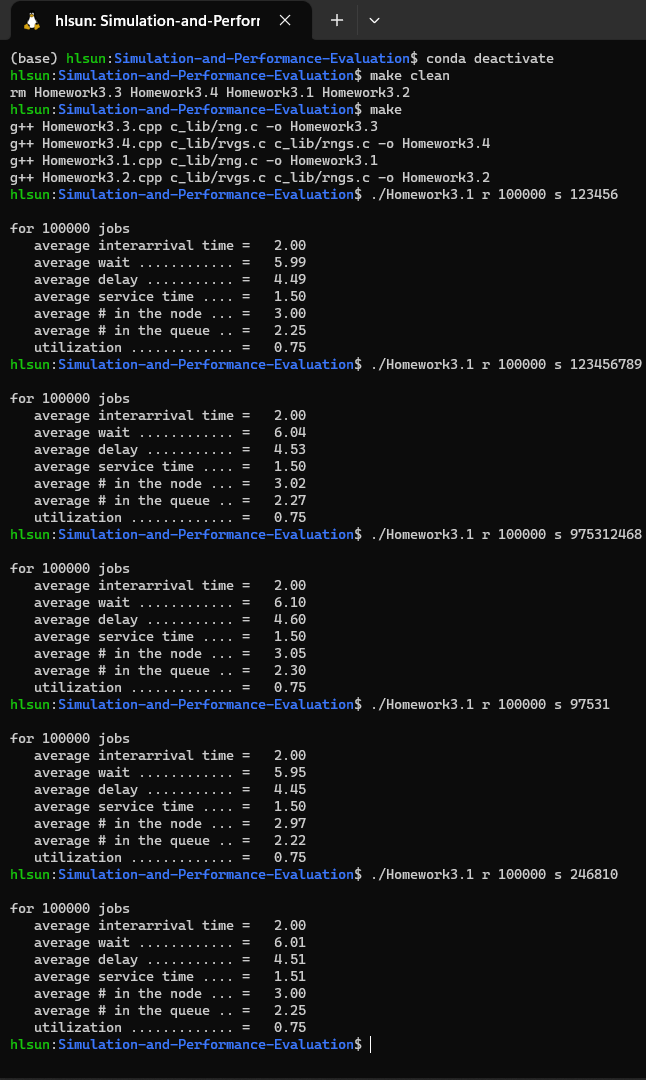
\includegraphics[scale=1]{Sections/Q1/H3_1.png}
\end{center}
\begin{lstlisting}[style=CStyle]
/**
 * Modified by Harrison Sun
 * sun.har@northeastern.edu
 * February 11, 2023
 */

/* -------------------------------------------------------------------------
 * This program - an extension of program ssq1.c - simulates a single-server
 * FIFO service node using Exponentially distributed interarrival times and
 * Uniformly distributed service times (i.e. a M/U/1 queue).
 *
 * Name              : ssq2.c  (Single Server Queue, version 2)
 * Author            : Steve Park & Dave Geyer
 * Language          : ANSI C
 * Latest Revision   : 9-11-98
 * -------------------------------------------------------------------------
 */

#include <exception>
#include <iostream>
#include <cstdlib>
#include <cstring>
#include <stdio.h>
#include <string>
#include <math.h>                                             
#include "c_lib/rng.h"

#define LAST         10000L                   /* number of jobs processed */ 
#define START        0.0                      /* initial time             */ 


double Exponential(double m)
/* ---------------------------------------------------
 * generate an Exponential random variate, use m > 0.0
 * ---------------------------------------------------
 */
{
    return (-m * log(1.0 - Random()));
}


double Uniform(double a, double b)
/* --------------------------------------------
 * generate a Uniform random variate, use a < b
 * --------------------------------------------
 */
{
    return (a + (b - a) * Random());
}


double GetArrival(void)
/* ------------------------------
 * generate the next arrival time
 * ------------------------------
 */
{
    static double arrival = START;

    arrival += Exponential(2.0);
    return (arrival);
}


//double GetService(void)
///* ------------------------------
// * generate the next service time
// * ------------------------------
// */
//{
//    return (Uniform(1.0, 2.0));
//}

/* Changing the GetService(void) function to return Exponential(1.5) service times */
double GetService(void)
{
    /* Generate the next service time */

    return (Exponential(1.5));
}

/* function to check if the input is a number */
bool checkArg(char* input)
{
    try 
    {
        if (strlen(input) > 9)
        {
            throw std::logic_error("Number is too large.");
        }

        for (int i = 0; i < strlen(input); ++i)
        {

            if (std::isdigit(input[i])) continue;
            else
            {
                std::string errorMessage;
                errorMessage.append((std::string)input);
                errorMessage.append(" is not a digit.");
                throw std::logic_error(errorMessage);
            }
        }
        return 1;
    }

    catch (const std::logic_error& error)
    {
        std::cerr << error.what() << std::endl;
        return 0;
    }
}

int main(int argc, char* argv[])
{
    long   index = 0;                         /* job index            */
    double arrival = START;                     /* time of arrival      */
    double delay;                                 /* delay in queue       */
    double service;                               /* service time         */
    double wait;                                  /* delay + service      */
    double departure = START;                     /* time of departure    */
    struct {                                      /* sum of ...           */
        double delay;                               /*   delay times        */
        double wait;                                /*   wait times         */
        double service;                             /*   service times      */
        double interarrival;                        /*   interarrival times */
    } sum = { 0.0, 0.0, 0.0 };

    long numRuns{};                                  /* number of runs */
    
    // Set the seed
    for (int i = 0; i < argc; ++i)
    {
        if (*argv[i] == 's' && checkArg(argv[i + 1]))
        {
            PutSeed(std::stol(argv[i + 1]));
            break;
        }
        else
        {
            PutSeed(123456789);
        }
    }

    // Set the number of runs
    for (int i = 0; i < argc; ++i)
    {
        if (*argv[i] == 'r' && checkArg(argv[i + 1]))
        {
            numRuns = std::stol(argv[i + 1]);
            break;
        }
        else
        {
            numRuns = 10000;
        }
    }
    
    while (index < numRuns) {
        index++;
        arrival = GetArrival();
        if (arrival < departure)
            delay = departure - arrival;         /* delay in queue    */
        else
            delay = 0.0;                         /* no delay          */
        service = GetService();
        wait = delay + service;
        departure = arrival + wait;              /* time of departure */
        sum.delay += delay;
        sum.wait += wait;
        sum.service += service;
    }
    sum.interarrival = arrival - START;

    printf("\nfor %ld jobs\n", index);
    printf("   average interarrival time = %6.2f\n", sum.interarrival / index);
    printf("   average wait ............ = %6.2f\n", sum.wait / index);
    printf("   average delay ........... = %6.2f\n", sum.delay / index);
    printf("   average service time .... = %6.2f\n", sum.service / index);
    printf("   average # in the node ... = %6.2f\n", sum.wait / departure);
    printf("   average # in the queue .. = %6.2f\n", sum.delay / departure);
    printf("   utilization ............. = %6.2f\n", sum.service / departure);

    return (0);
}

\end{lstlisting}
\pagebreak

\section{\textbf{Ex. 3.1.5}}
\textbf{(a) Verify that the mean service time in Example 3.1.4 is 1.5.}\\
\textbf{(b) Verify that the steady-state statistics in Example 3.1.4 seem to be correct.}\\
\textbf{(c) Note that the arrival rate, service rate, and utilization are the same as those in Example 3.1.3. Explain (or conjecture) why this is so. Be Specific.}\\
\begin{center}
\includegraphics[scale=0.75]{Sections/Q2/3.1.3.png}\\
\vspace{10pt}
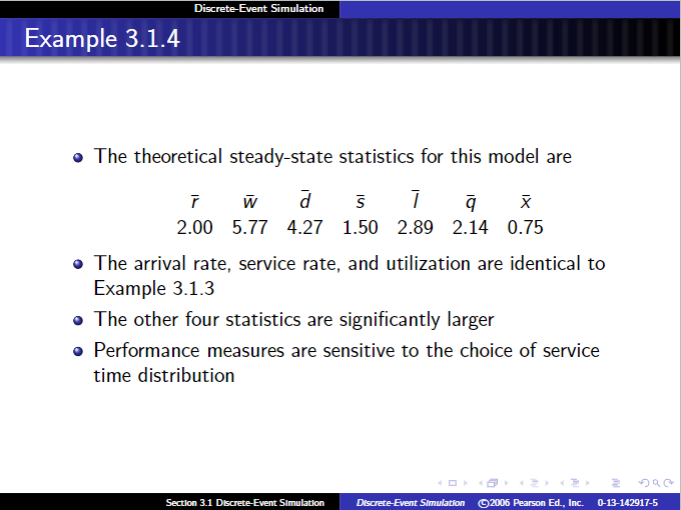
\includegraphics[scale=0.75]{Sections/Q2/3.1.4.png}\\
\end{center}
\newpage
\vspace{35pt}
\begin{center}
    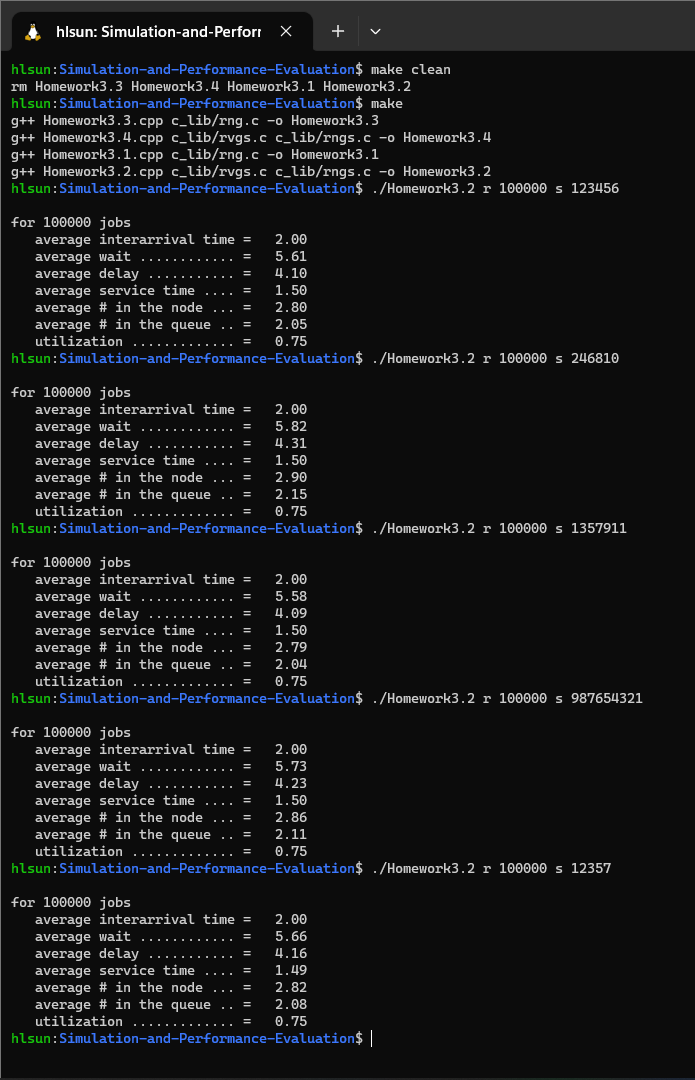
\includegraphics[scale=0.75]{Sections/Q2/H3_2.png}
\end{center}
\newpage
\begin{table}[h]
\centering
\begin{tabular}{l|lllll}
                  & 123456 & 246810 & 1357911 & 987654321 & 12357 \\
                  \hline\\
interarrival time & 2.00   & 2.00   & 2.00    & 2.00      & 2.00  \\
wait time         & 5.61   & 5.82   & 5.58    & 5.73      & 5.66  \\
delay time        & 4.10   & 4.31   & 4.09    & 4.23      & 4.16  \\
service time      & 1.50   & 1.50   & 1.50    & 1.50      & 1.49  \\
number in node    & 2.80   & 2.90   & 2.79    & 2.86      & 2.82  \\
number in queue   & 2.05   & 2.15   & 2.04    & 2.11      & 2.08  \\
utilization       & 0.75   & 0.75   & 0.75    & 0.75      & 0.75 
\end{tabular}
\end{table}
\noindent The arrival rate is the same because the interarrival time is defined by the same distribution as in Example 3.1.3: $r \sim Exponential(2.0)$.\\\\

\noindent The average service rate is the same as in Example 3.1.3 due to the distribution of the service times. The average number of tasks $\Bar{t}$ of $t \sim 1+ Geometric(0.9)$ is $1$ plus the inverse of $p=0.9$. Therefore, the average number of tasks is 10. The average of $Uniform(0.1, 0.2)$ is $0.15$. Multiplying this and the number of tasks together results in an average service rate $\Bar{s} = 1.5$, which is the same as the service rate in Example 3.1.3.\\\\

\noindent The server utilization is the same as in Example 3.1.3 because the average interarrival times and average service rates are the same in both examples. The server utilization is a ratio of the interarrival and service time averages.

\newpage
\begin{lstlisting}[style=CStyle]
/**
 * Homework 3.2
 * EECE 5643 - Simulation and Performance Evaluation
 * Author: Harrison Sun
 * Email: sun.har@northeastern.edu
 */

#include <cstdlib>
#include <cstring>
#include <stdio.h>
#include <exception>
#include <iostream>
#include <math.h> 
#include <string>
#include "c_lib/rvgs.h"
#include "c_lib/rngs.h"

#define LAST         10000L                   /* number of jobs processed */
#define START        0.0                      /* initial time             */

 /**
  * double GetArrival()
  *
  * @param void
  * @return arrival - the next arrival time
  *
  * This function calculates the arrival times for each process.
  */

double GetArrival()
{
    static double arrival = START;

    arrival += Exponential(2.0);
    return (arrival);
}


/**
 * double GetService()
 *
 * @param void
 * @return sum - the total service time for the process
 *
 * This function calculates the service times for each process.
 */

double GetService()
{
    long k{};
    double sum{ 0.0 };
    long tasks = 1 + Geometric(0.9);
    for (k = 0; k < tasks; ++k)
    {
        sum += Uniform(0.1, 0.2);
    }
    return sum;
}

/**
 * bool checkArg()
 *
 * @param char* input - the input string literal from the console
 * @return bool - true if the input is a number, false otherwise
 *
 * This function determines whether the argument is a number.
 */

bool checkArg(char* input)
{
    try
    {
        if (strlen(input) > 9)
        {
            throw std::logic_error("Number is too large.");
        }

        for (int i = 0; i < strlen(input); ++i)
        {

            if (std::isdigit(input[i])) continue;
            else
            {
                std::string errorMessage;
                errorMessage.append((std::string)input);
                errorMessage.append(" is not a digit.");
                throw std::logic_error(errorMessage);
            }
        }
        return 1;
    }

    catch (const std::logic_error& error)
    {
        std::cerr << error.what() << std::endl;
        return 0;
    }
}

/**
 * int main()
 *
 * @param int argc - the number of arguments
 * @param char* argv[] - the arguments
 *
 * @return int - 0 if the program runs successfully
 */

int main(int argc, char* argv[])
{
    long   index = 0;                         /* job index            */
    double arrival = START;                     /* time of arrival      */
    double delay;                                 /* delay in queue       */
    double service;                               /* service time         */
    double wait;                                  /* delay + service      */
    double departure = START;                     /* time of departure    */
    struct {                                      /* sum of ...           */
        double delay;                               /*   delay times        */
        double wait;                                /*   wait times         */
        double service;                             /*   service times      */
        double interarrival;                        /*   interarrival times */
    } sum = { 0.0, 0.0, 0.0 };

    long numRuns{};                                  /* number of runs */

    // Set the seed
    for (int i = 0; i < argc; ++i)
    {
        if (*argv[i] == 's' && checkArg(argv[i + 1]))
        {
            PutSeed(std::stol(argv[i + 1]));
            break;
        }
        else
        {
            PutSeed(123456789);
        }
    }

    // Set the number of runs
    for (int i = 0; i < argc; ++i)
    {
        if (*argv[i] == 'r' && checkArg(argv[i + 1]))
        {
            numRuns = std::stol(argv[i + 1]);
            break;
        }
        else
        {
            numRuns = 10000;
        }
    }

    while (index < numRuns) {
        index++;
        arrival = GetArrival();
        if (arrival < departure)
            delay = departure - arrival;         /* delay in queue    */
        else
            delay = 0.0;                         /* no delay          */
        service = GetService();
        wait = delay + service;
        departure = arrival + wait;              /* time of departure */
        sum.delay += delay;
        sum.wait += wait;
        sum.service += service;
    }
    sum.interarrival = arrival - START;

    printf("\nfor %ld jobs\n", index);
    printf("   average interarrival time = %6.2f\n", sum.interarrival / index);
    printf("   average wait ............ = %6.2f\n", sum.wait / index);
    printf("   average delay ........... = %6.2f\n", sum.delay / index);
    printf("   average service time .... = %6.2f\n", sum.service / index);
    printf("   average # in the node ... = %6.2f\n", sum.wait / departure);
    printf("   average # in the queue .. = %6.2f\n", sum.delay / departure);
    printf("   utilization ............. = %6.2f\n", sum.service / departure);
    return 0;
}
\end{lstlisting}
\pagebreak

\section{\textbf{Ex. 3.3.1}}
\textbf{Suppose that each die in a pair of dice is loaded (unfair) in such a way that the
6-face is four times as likely as the opposite 1-face and each of the other four faces are twice as likely as the 1-face.\\\\}
\pagebreak

\section{\textbf{Ex. 3.3.4}}
\textbf{(a) Construct a continuous-data histogram of the service times (in ac.dat - Exercise 1.2.6).\\
(b) Compare the histogram mean and standard deviation with the corresponding sample mean and standard deviation, and justify your choice of histogram parameters $a$, $b$, and either $k$ or $\delta$.}\\\\
\noindent Terminal Output\\
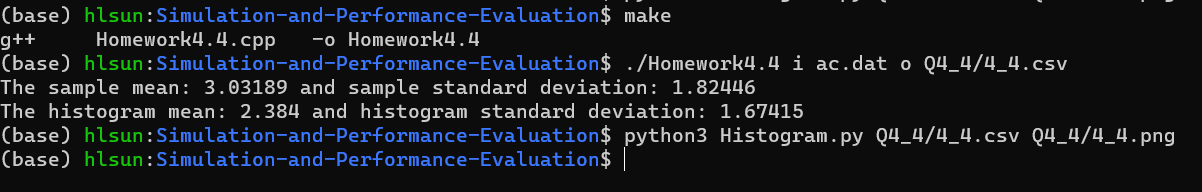
\includegraphics[scale=0.6]{Sections/Q4/4_4_terminal.png}\\

\noindent The sample mean: 3.03\\
The sample standard deviation: 1.82\\
The histogram mean: 3.03\\
The histogram standard deviation: 1.81\\\\

\noindent We can see that the sample and histogram mean and standard deviation are similar. This means that the number of bins used was sufficient to ensure an accurate representation of the data. Additionally, the histogram is mostly smooth, meaning the number of bins used was not excessively high in order to achieve this sample statistic performance. \\\\

\noindent a and b were chosen to be the minimum and maximum values, as this allows the histogram to fit all of the data while also not allocating bins for data outside the range. The number of bins was chosen such that $k \in [\lfloor ln(n) \rfloor, \lfloor\sqrt{n}\rfloor]$. Given that $n = 500$, $k \in [6,22]$. 18 was chosen because more bins than the minimum were needed knowing that outlier data is significantly larger than the mean. This can been seen in the histogram below, where there are several empty bins before reaching the maximum bin. However, setting $k$ too high, such as $k=22$ would result in a noisy histogram. Therefore, it was decided that $k=18$.\\\\

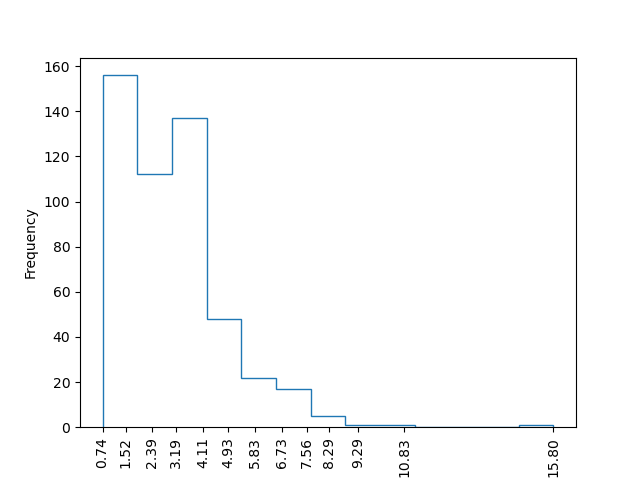
\includegraphics[scale=1]{Sections/Q4/4_4.png}
\newpage
\begin{lstlisting}[style=CStyle]
/**
 * Harrison Sun (sun.har@northeastern.edu)
 * EECE 5643 - Simulation and Performance Evaluation
 * Homework 4.4
 */

#define DEFAULT_IFILE		"ac.dat"
#define DEFAULT_OFILE		"output.txt"

#include <algorithm>
#include <cstdlib>
#include <cstring>
#include <fstream>
#include <stdio.h>
#include <exception>
#include <iostream>
#include <list>
#include <math.h> 
#include <string>
#include <vector>
#include "c_lib/rvgs.h"
#include "c_lib/rngs.h"
#include "checkarg/checkarg.h"

void sortDataIntoBins(const std::vector<double>& data, int numBins, std::vector<std::pair<double, long>>& meanOfBinAndCount) {
	// Initialize the meanOfBinAndCount vector with empty bins and counts of 0
	meanOfBinAndCount.clear();
	for (int i = 0; i < numBins; i++) {
		meanOfBinAndCount.push_back(std::make_pair(0.0, 0));
	}

	// Find the range of the data
	double minData = *std::min_element(data.begin(), data.end());
	double maxData = *std::max_element(data.begin(), data.end());
	double range = maxData - minData;

	// Calculate the width of each bin
	double binWidth = range / numBins;

	// Sort the data into bins and update the mean and count of each bin
	for (int i = 0; i < data.size(); i++) {
		// Determine which bin the data point belongs to
		int binIndex = std::min(static_cast<int>((data[i] - minData) / binWidth), numBins - 1);

		// Update the mean and count of the bin
		double binMean = meanOfBinAndCount[binIndex].first;
		long binCount = meanOfBinAndCount[binIndex].second;
		binMean = (binMean * binCount + data[i]) / (binCount + 1);
		binCount++;
		meanOfBinAndCount[binIndex] = std::make_pair(binMean, binCount);
	}
}



/**
 * int main() - The main function
 *
 * @param int argc - the number of arguments
 * @param char* argv[] - the arguments
 *
 * @return 0 if the program runs successfully
 * 
 * This is the main function. It reads in a data file in tab separated format. The first column contains the arrival times and the second column
 * contains departure times.
 * 
 */

int main(int argc, char* argv[])
{
	// Create two vectors to store the data
	std::vector<double> arrival_times{};
	std::vector<double> departure_times{};
	std::vector<double> service_times{};

	// Histogram Parameters
	int nHistogram { 500 }; // The number of jobs in the data file
	// The number of bins in the histogram. Ideally, k ~ [ln(n), sqrt(n)] => Choosing from k ~ [6, 22]
	
	/*****************************************************************************************************************************************************************

		The number of bins is chosen to be 18 This is significantly larger than the minimum k = 6. The reason for this choice is that the service times are empirical 
		data and may have significant outliers that would not fit well with other data when given too few bins. However, 22 bins would be too many, as the data has
		high variance and would thus have a lot of empty bins. 18 bins is a good compromise between the two.
		
	*****************************************************************************************************************************************************************/
	
	int nBins{18};
	
	// File names
	std::string inputFileName{};
	std::string outputFileName{};

	// Set the input file stream
	for (int i = 0; i < argc; ++i)
	{
		if (*argv[i] == 'i')
		{
			inputFileName = argv[i + 1];
			break;
		}
		else
		{
			inputFileName = DEFAULT_IFILE;
		}
	}
	
	// Set the output file stream
	for (int i = 0; i < argc; ++i)
	{
		if (*argv[i] == 'o')
		{
			outputFileName = argv[i + 1];
			break;
		}
		else
		{
			outputFileName = DEFAULT_OFILE;
		}
	}
	
	double arrival_time{};
	double departure_time{};
	
	std::ifstream infile;
	infile.open(inputFileName.c_str());
	
	// Read in the data from the tsv to the vectors
	while (infile >> arrival_time >> departure_time)
	{
		arrival_times.push_back(arrival_time);
		departure_times.push_back(departure_time);
	}
	infile.close();
	
	// Calculate the service times and store them in the service_times vector
	for (int i = 0; i < arrival_times.size(); ++i)
	{
		// Check if the service node is free at arrival
		if (arrival_times[i] > departure_times[i - 1])
		{
			service_times.push_back(departure_times[i] - arrival_times[i]);
		}
		// If the job has to wait in a queue, the service starts after the previous job is finished
		else
		{
			service_times.push_back(departure_times[i] - departure_times[i - 1]);
		}
	}

	// Calculate the total service time
	double total_service_time{};
	for (std::vector<double>::iterator i = service_times.begin(); i != service_times.end(); ++i)
	{
		total_service_time += *i;
	}
	
	// Calculate the sample mean and standard deviation
	double sample_mean{ total_service_time / service_times.size() };
	double sample_std{};
	
	// Standard Deviation
	for (std::vector<double>::iterator i = service_times.begin(); i != service_times.end(); ++i)
	{
		sample_std += pow(*i - sample_mean, 2);
	}
	sample_std = sqrt(sample_std / (service_times.size() - 1));

	// Vector to store the bin information as a pair
	std::vector<std::pair<double, long>> BinVector;

	// Call the function to sort the data into bins
	sortDataIntoBins(service_times, nBins, BinVector);

	// Store the bin means and counts in output file
	std::ofstream outfile;
	outfile.open(outputFileName.c_str());
	
	for (int i = 0; i < nBins; ++i)
	{
		outfile << BinVector[i].first << ", " << BinVector[i].second << std::endl;
	}
	
	outfile.close();
	
	// Calculate the histogram mean and standard deviation
	double histogram_mean{};
	double histogram_std{};
	
	for (int i = 0; i < nBins; ++i)
	{
		histogram_mean += BinVector[i].first * BinVector[i].second;
	}
	
	histogram_mean /= nHistogram;
	
	for (int i = 0; i < nBins; ++i)
	{
		histogram_std += BinVector[i].second * pow(BinVector[i].first - histogram_mean, 2);
	}
	
	histogram_std = sqrt(histogram_std / (nHistogram - 1));
	
	// Output the means and standard deviations
	std::cout << "The sample mean: " << sample_mean << " and sample standard deviation: " << sample_std << std::endl;
	std::cout << "The histogram mean: " << histogram_mean << " and histogram standard deviation: " << histogram_std << std::endl;
	return 0;
}
\end{lstlisting}
\end{document}
